\section{Stream computations}\label{sec:streams}

The core notion of \dbsp is the \textbf{stream}.  In this section we
introduce streams, and several structured ways of computing on
streams.  Stream operators are the basic building block of stream
computations; operators can be composed into complex computational
circuits.

\subsection{Streams and stream operators}\label{sec:notation}

%\begin{definition}[stream]
Given a set $A$, a \defined{stream} \emph{of values from $A$} is an
infinite sequence of values from $A$.  We write $\stream{A}$ is the
set of all streams with value from $A$.
%\end{definition}
We write $s[t]$ for the $t$-th element of the stream $s$.  Think of
$t$ as the ``time'' and of $s[t]\in A$ as the value of the the stream
$s$ ``at time'' $t$.  We show streams as a sequence of boxes: e.g.,
the stream $s[t] = t$ is \sv{0 1 2 3 4}.

%\begin{definition}[stream operator]
A \defined{stream operator} is a function that computes on streams and
produces streams.
%\end{definition}
In general we use ``operator'' for streams, and ``function'' for
computations on ``scalar'' values.

In this paper we mostly use circuit diagrams to depict \dbsp
programs\footnote{Circuits hide the \emph{order} of the inputs of an
operator.}.  In a circuit a rectangle represents an operator (and is
labeled with the operator name, e.g., $T$), while an arrow with a
double head is a stream.  Please note that this notation differs from
the one in the original paper~\cite{budiu-vldb23}, where we used
single arrows for stream in most cases.

Stream operator can be composed, as in this example:

\begin{center}
\begin{tikzpicture}[auto,>=latex]
  \node[] (input) {$s$};
  \node[] [right of=input] (dummy) {};
  \node[block, below of=dummy, node distance=.7cm] (S1) {$S$};
  \node[block, right of=S1] (T1) {$T$};
  \node[block, right of=T1] (T2) {$T$};
  \node[block, above of=T2, node distance=.7cm] (S2) {$S$};
  \node[right of=T2] (output) {$o$};
  \draw[->>] (input) -| (S1);
  \draw[->>] (input) -| (T1);
  \draw[->>] (S1) -- (T1);
  \draw[->>] (T1) -- (T2);
  \draw[->>] (input) |- (S2);
  \draw[->>] (T2) -- (output);
  \draw[->>] (S2) -- (T2);
\end{tikzpicture}
\end{center}

%\begin{definition}(lifting)
Given a function $f: A \to B$, we define a stream operator $\lift{f}
:\stream{A} \to \stream{B}$ (read as $f$ lifted) by applying function
$f$ to the input stream(s) independently at each point in time.
\begin{center}
  \begin{tikzpicture}[auto,>=latex]
    \node[] (input) {$\sv{a b c d e}$};
    \node[block, right of=input, node distance=2.2cm] (f) {$\lift{f}$};
    \node[right of=f, node distance=2.8cm] (output) {$\sv{f(a) f(b) f(c) f(d) f(e)}$};
    \draw[->>] (input) -- (f);
    \draw[->>] (f) -- (output);
  \end{tikzpicture}
\end{center}
%\end{definition}

We say that two \dbsp programs are \defined{equivalent} if they
compute the same input-output function on streams.  We use the symbol
$\cong$ to indicate circuit equivalence.  For example, we
can prove the following circuit equivalence (where $\circ$ is function
composition):

\noindent
\begin{tabular}{m{3.5cm}m{.3cm}m{3.5cm}}
\begin{tikzpicture}[auto,>=latex]
  \node[] (input) {$s$};
  \node[block, right of=input] (g) {$\lift{g}$};
  \node[block, right of=g] (f) {$\lift{f}$};
  \node[right of=f] (output) {$o$};
  \draw[->>] (input) -- (g);
  \draw[->>] (g) -- (f);
  \draw[->>] (f) -- (output);
\end{tikzpicture}
&
$\cong$
&
\begin{tikzpicture}[auto,>=latex]
    \node[] (input) {$s$};
    \node[block, right of=input, node distance=1.5cm] (fg) {$\lift{(f \circ g)}$};
    \node[right of=fg, node distance=1.5cm] (output) {$o$};
    \draw[->>] (input) -- (fg);
    \draw[->>] (fg) -- (output);
\end{tikzpicture}
\end{tabular}

To simplify the notation, we will write $a + b$ for streams $a, b$
instead of $a (\lift{+}) b$; we will also write $-a$ instead of
$(\lift{-})a$.

\subsection{Useful stream operators}\label{sec:abelian}

For the rest of this paper we require the set of values $A$ of a
stream $\stream{A}$ to form a commutative group, with operations $+$,
$-$, and a $0$ (zero) value.  The \emph{plus} defines what it means to
\emph{add} new data, while the \emph{minus} allows us to compute
differences (deltas).  We show later that this requirement is not a
problem for using \dbsp in the context of databases.

%\subsubsection{Delays}\label{sec:delay}

%\begin{definition}[Delay]
The \defined{delay operator} $z^{-1}$ produces an output stream by
delaying its input by one step (and starting with a
zero)\footnote{This bizarre name comes from digital signal
processing.}:

  \begin{center}
  \begin{tikzpicture}[auto,>=latex,node distance=2.4cm]
    \node[] (input) {$\sv{a b c d e}$};
    \node[block, right of=input] (z) {$z^{-1}$};
    \node[right of=z] (output) {$\sv{0 a b c d}$};
    \draw[->>] (input) -- (z);
    \draw[->>] (z) -- (output);
  \end{tikzpicture}
  \end{center}
%\end{definition}

%\begin{definition}[Time invariance]
%A stream operator $S: \stream{A} \to \stream{B}$ is \defined{time-invariant} (TI) if
%$S(\zm_A(s)) = \zm_B(S(s))$ for all $s \in \stream{A}$; in other words, if
%the following two circuits are equivalent:
%
%\begin{tabular}{m{3cm}m{.5cm}m{3cm}}
%\begin{tikzpicture}[auto,>=latex]
%  \node[] (input) {$s$};
%  \node[block, right of=input] (S) {$S$};
%  \node[block, right of=S] (z) {$\zm$};
%  \node[right of=z] (output) {$o$};
%  \draw[->] (input) -- (S);
%  \draw[->] (S) -- (z);
%  \draw[->] (z) -- (output);
%\end{tikzpicture}
%&
%$\cong$
%&
%\begin{tikzpicture}[auto,>=latex]
%  \node[] (input) {$s$};
%  \node[block, right of=input] (z) {$\zm$};
%  \node[block, right of=z] (S) {$S$};
%  \node[right of=S] (output) {$o$};
%  \draw[->] (input) -- (z);
%  \draw[->] (z) -- (S);
%  \draw[->] (S) -- (output);
%\end{tikzpicture}
%\end{tabular}
%
%\noindent
%This definition extends
%naturally to operators with multiple inputs.
%\end{definition}
%
%The composition of TI operators of any number of inputs
%is TI. The delay operator $\zm$ is TI.
%\dbsp only uses TI operators.
%
%%\begin{definition}
%%We say that a function between groups $f: A \to B$ has the \emph{zero-preservation
%%property} if $f(0_A) = 0_B$.  We write $\zpp{f}$.
%%\end{definition}
%%
%%A lifted operator $\lift{f}$ is TI iff $\zpp{f}$.
%
%\subsubsection{Causal and strict operators}\label{sec:causal}
%
%\begin{definition}[Causality]
%A stream operator $S:\stream{A}\to\stream{B}$
%is \defined{causal} when for all $s,s'\in\stream{A}$,
%and all times $t$ we have:
%$
%(\forall i \leq t . s[i]=s'[i]) ~~\Rightarrow~~ S(s)[t]=S(s')[t].
%$
%\end{definition}
%
%\noindent
%In other words, the output value at time $t$ can only depend on
%input values from times $t' \leq t$.
%Operators produced by lifting are causal, and $\zm$ is causal.
%All \dbsp operators are causal.  The composition
%of causal operators of any number of inputs is causal.
%
%\begin{definition}[Strictness]
%A stream operator, $F:\stream{A}\to\stream{B}$
%is \defined{strict}
%if  $\forall s,s'\in\stream{A}, \forall t \in \N$ we have:
%$(\forall i<t . ~s[i]=s'[i]) ~~\Rightarrow \\ F(s)[t]=F(s')[t].$
%\end{definition}
%
%In other words, the $t$-th output of $F(s)$ can depend only on ``past'' values
%of the input $s$, between $0$ and $t-1$.
%In particular, $F(s)[0] = 0_B$ is the same for all $s \in \stream{A}$.
%Strict operators are causal. Lifted operators in general are \emph{not} strict.
%$\zm$ is strict.  %In \dbsp $\zm$ is the only primitive strict operator.
%
%\begin{proposition}
%\label{prop-unique-fix}
%For a strict $F: \stream{A} \to \stream{A}$ the equation ~$\alpha=F(\alpha)$~ has a unique
%solution $\alpha \in \stream{A}$, denoted by $\fix{\alpha}{F(\alpha)}$.
%\end{proposition}
%
%Thus every strict operator from a set to itself has a unique fixed
%point.  The simple proof relies on strong induction, showing that the
%solution $\alpha[t]$ depends only on the values of $\alpha$ prior to
%$t$.
%
%Consider a circuit with a strict feedback edge:
%\begin{center}
%\begin{tikzpicture}[>=latex]
%    \node[] (input) {$s$};
%    \node[block, right of=input] (f) {$T$};
%    \node[right of=f] (output) {$\alpha$};
%    \node[block, below of=f, node distance=.5cm] (z) {$F$};
%    \draw[->] (input) -- (f);
%    \draw[->] (f) -- node (mid) {} (output);
%    \draw[->] (mid.center) |-  (z);
%    \draw[->] (z.west) -- ++(-.3,0) |- ([yshift=1mm]f.south west);
%\end{tikzpicture}
%\end{center}
%
%This circuit is a well-defined function on streams:
%
%%\begin{lemma}
%%\label{lemma-causal-strict}
%%If $F: \stream{B} \to \stream{B}$ is strict and $T: \stream{A} \times \stream{B} \to \stream{B}$ is causal, then for fixed $s$ the operator
%%$\lambda\alpha.T(s,F(\alpha)): \stream{A} \to \stream{B}$ is strict.
%%\end{lemma}
%
%\begin{lemma}\label{feedback-semantics}
%\label{cor-loop}
%If $F: \stream{B} \to \stream{B}$ is strict and $T: \stream{A} \times \stream{B} \to \stream{B}$ is causal,
%the operator $Q(s)=\fix{\alpha}{T(s,F(\alpha))}$ is well-defined and causal.
%If, moreover, $F$ and $T$ are TI then so is $Q$.
%\end{lemma}
%
%All \dbsp computations are built using just lifted functions and
%delays.  We add two more operators in \secref{sec:nested}.
%
%\subsection{Integration and differentiation}\label{sec:abelianstreams}

%Remember that we require the elements of a stream to come from an abelian group $A$.
%Streams themselves form an abelian group:
%
%\begin{proposition}
%The structure $(\stream{A},+,0,-)$, obtained by lifting the $+$ and unary $-$ operations of $A$,
%is an abelian group.  0 is the stream with all values $0_A$.
%\end{proposition}
%
%\noindent
%Stream addition and negation are causal, TI operators.

%Given a linear function $f: A \to B$, the stream operator $\lift{f}$
%is linear and TI (LTI).  $\zm$ is also LTI.
%
%\begin{definition}(bilinear)
%A function of two arguments $f: A \times B \to C$ with $A, B, C$ groups, is \emph{bilinear}
%if it is linear separately in each argument (i.e., it distributes over addition):
%$\forall a, b, c, d . f(a+b, c) = f(a, c) + f(b, c)$, and $f(a, c+d) = f(a, c) + f(c, d).$
%\end{definition}
%
%This definition extends to stream operators.
%The lifting of a bilinear function $f$ is
%a bilinear stream operator $\lift{f}$.  An example
%is lifted multiplication:
%$f: \stream{\N} \times \stream{\N} \to \stream{\N}, f(a, b)[t] = a[t]\cdot b[t]$.

%The composition of (bi)linear operators with linear operators
%is (bi)linear (since homomorphisms compose).

%The ``feedback loop'' of a linear operator is linear:
%
%\begin{proposition}
%\label{prop-rec-linear}
%Let $S$ be a unary, causal, LTI operator. The
%operator $Q(s)=\fix{\alpha}{S(s+\zm(\alpha))}$ is well-defined and LTI:
%
%\begin{center}
%\begin{tikzpicture}[>=latex]
%    \node[] (input) {$s$};
%    \node[block, shape=circle, right of=input, inner sep=0pt, node distance=.6cm] (plus) {$+$};
%    \node[block, right of=plus, node distance=.6cm] (Q) {$S$};
%    \node[right of=Q, node distance=1.2cm] (output) {$\alpha$};
%    \node[block, below of=Q, node distance=.6cm] (z) {$\zm$};
%    \draw[->] (input) -- (plus);
%    \draw[->] (plus) -- (Q);
%    \draw[->] (Q) -- node (mid) {} (output);
%    \draw[->] (mid.center) |-  (z);
%    \draw[->] (z) -| (plus);
%\end{tikzpicture}
%\end{center}
%\end{proposition}

%\begin{definition}[Differentiation]
We can define \defined{differentiation operator} as a composition of
several other operators: $\D(s) \defn s - \zm(s)$, show as:

\begin{center}
\begin{tikzpicture}[auto,>=latex,node distance=1cm]
    \node[] (input) {$s$};
    \node[block, shape=circle, right of=input, inner sep=0pt,node distance=2cm] (plus) {$+$};
    \node[right of=plus] (output) {$\D(s)$};
    \draw[draw,->] (input) -- node (i) {} (plus);
    \node[block, below of=i, node distance=.8cm] (z) {$\zm$};
    \node[block, shape=circle, right of=z, inner sep=1pt] (minus) {$-$};
    \draw[->>] (plus) -- (output);
    \draw[->>] (i) -- (z);
    \draw[->>] (z) -- (minus);
    \draw[->>] (minus) -- (plus);
\end{tikzpicture}
\end{center}
%\end{definition}
%We generally omit the type, and write just $\D$.
%The value of $\D(s)[t] = s[t] - s[t-1]$ if $t > 0$.

If $s$ is a stream, then $\D(s)$ is the \emph{stream of changes} of
$s$; a value in the output is the difference between two consecutive
values in the input.  As an example, $\D(\sv{0 1 2 3 4 5}) = \sv{0 1 1
  1 1}$.

%\begin{proposition}
%\label{prop-diff-properties}
%$\D$ is causal and LTI.
%\end{proposition}

%The integration operator ``reconstitutes'' a stream from its changes:

%\begin{definition}[Integration]
The \defined{integration operator}
is given by the following circuit:
\begin{center}
\begin{tikzpicture}[auto,>=latex, node distance=1.1cm]
    \node[] (input) {s};
    \node[block, shape=circle, right of=input, inner sep=0pt] (plus) {$+$};
    \node[right of=plus, node distance=1.6cm] (output) {$\I(s)$};
    \node[block, below of=plus, node distance=.8cm] (z) {$z^{-1}$};
    \draw[->>] (input) -- (plus);
    \draw[->>] (plus) -- node (o) {} (output);
    \draw[->>] (o) |- (z);
    \draw[->>] (z) -- (plus);
\end{tikzpicture}
\end{center}
%\end{definition}

While this definition may seem strange, because the output stream is
used to compute itself, the use of the delay in the ``feedback'' loop
ensures that only ``previous'' values of the output are used in
computing the current one, so this circuit is really well-defined.
%\noindent
%We also generally omit the type, and write just $\I$.
%This is the construction from Proposition~\ref{prop-rec-linear}
%using the identity function for $S$.
%
%\begin{proposition}
%$\I(s)$ is the discrete (indefinite) integral applied to the stream $s$:
%\end{proposition}
In general, $\I(s)[t] = \sum_{i \leq t} s[i]$.
As an example, $\I(\sv{0 1 2 3 4 5}) = \sv{0 1 3 6 10}$.

%\begin{proposition}
%\label{prop-integ-properties}
%$\I$ is causal and LTI.
%\end{proposition}
%
%\begin{theorem}[Inversion]
%\label{inverses}
%Integration and differentiation are inverses of each other:
%$\forall s . \I(\D(s)) = \D(\I(s)) = s$.
%\end{theorem}

Integration and differentiation ``cancel'' each other:

\noindent
\begin{tabular}{m{2.5cm}m{.3cm}m{1cm}m{.3cm}m{2.5cm}}
\begin{tikzpicture}[auto,>=latex, node distance=.75cm]
    \node[] (input) {$s$};
    \node[block, right of=input] (I) {$\I$};
    \node[block, right of=I] (D) {$\D$};
    \node[right of=D] (output) {$o$};
    \draw[->>] (input) -- (I);
    \draw[->>] (I) -- (D);
    \draw[->>] (D) -- (output);
\end{tikzpicture}
     &
     $\cong$
     &
     \hspace{-2ex}
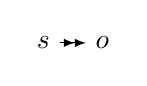
\begin{tikzpicture}[auto,>=latex, node distance=.75cm]
    \node[] (input) {$s$};
    \node[right of=input] (output) {$o$};
    \draw[->>] (input) -- (output);
\end{tikzpicture}
     &
     $\cong$
     &
\begin{tikzpicture}[auto,>=latex, node distance=.75cm]
    \node[] (input) {$s$};
    \node[block, right of=input] (D) {$\D$};
    \node[block, right of=D] (I) {$\I$};
    \node[right of=I] (output) {$o$};
    \draw[->>] (input) -- (D);
    \draw[->>] (D) -- (I);
    \draw[->>] (I) -- (output);
\end{tikzpicture}
\end{tabular}

\section{Incremental view maintenance}\label{sec:incremental}

%Here we define IVM and analyze its properties.

%\begin{definition}
Given a stream operator $Q: \stream{A} \to \stream{B}$ we define the
\defined{incremental version} of $Q$ as:
%\begin{equation}\label{def:inc}
%\inc{Q} \defn \D \circ Q \circ \I.
%\end{equation}
%$\inc{Q}$ has the same ``type'' as $Q$: $\inc{Q}: \stream{A} \to \stream{B}$.
%For an operator with multiple inputs we define
%the incremental version by applying $\I$ to each input independently:
%e.g., if $T: \stream{A} \times \stream{B} \rightarrow \stream{C}$ then
%$\inc{T}(a, b) \defn \D (T(\I(a), \I(b)))$.

%The following diagram illustrates the intuition behind this
%definition:
\vspace{-2ex}
\begin{center}
\begin{tikzpicture}[auto,>=latex]
    \node[] (input) {$\Delta s$};
    \node[block, right of=input] (I) {$\I$};
    \node[block, right of=I] (Q) {$Q$};
    \node[block, right of=Q] (D) {$\D$};
    \node[right of=D] (output) {$\Delta o$};
    \draw[->>] (input) -- (I);
    \draw[->>] (I) -- node (s) {$s$} (Q);
    \draw[->>] (Q) -- node (o) {$o$} (D);
    \draw[->>] (D) -- (output);
    \draw[decorate, decoration = {brace, raise=13pt}] (input) -- (output)
    node[pos=.5, above=13pt]{$\inc{Q}$};
\end{tikzpicture}
\end{center}
%\end{definition}

If $Q$ computes on a stream $s$, then $\inc{Q}$ computes on a stream
of changes to $s$.  If $Q$ produces a stream $o$, then $\inc{Q}$
produces the stream of changes to $o$.
%Notice that our definition of incremental computation is meaningful only for \emph{streaming}
%computations; this is in contrast to classic definitions, e.g.~\cite{gupta-idb95} which
%consider only one change.  Generalizing the definition to operate on streams gives us
%additional power, especially when operating with recursive queries.
%
%The following proposition is one of our central results:
$\inc{Q}$ has many nice properties:

%\begin{proposition}(Properties of the incremental version):
%\label{prop-inc-properties}
%\begin{description}
%\item[inversion:] $Q\mapsto\inc{Q}$ is bijective; its inverse is $Q\mapsto \I\circ Q\circ\D$.
%\item[invariance:] $\inc{+} = +, \inc{(\zm)} = \zm, \inc{-} = -, \inc{\I}=\I, \inc{\D}=\D$
%\item[push/pull:] \label{prop-part-commutation}
%    $Q \circ \I = \I \circ \inc{Q}$; $\D\circ Q = \inc{Q}\circ\D$
%\item[chain:] $\inc{(Q_1\circ Q_2)} = \inc{Q_1}\circ\inc{Q_2}$ (Generalizes to multiple inputs.)
%\item[add:] $\inc{(Q_1 + Q_2)} = \inc{Q_1} + \inc{Q_2}$
%\item[cycle:] $\inc{(\lambda s. \fix{\alpha}{T(s,\zm(\alpha)}))} = \lambda s. \fix{\alpha}{\inc{T}(s,\zm(\alpha)})$
%\end{description}
%\end{proposition}
%
The \defined{chain rule} states that $\inc{(Q_1 \circ Q_2)} =
\inc{Q_1} \circ \inc{Q_2}$, i.e., these circuits are equivalent:

\noindent
\begin{tabular}{rr}
\begin{tikzpicture}[auto,>=latex]
  \node[] (input) {$\Delta i$};
  \node[block, right of=input] (I) {$\I$};
  \node[block, right of=I] (Q1) {$Q_1$};
  \node[block, right of=Q1] (Q2) {$Q_2$};
  \node[block, right of=Q2] (D) {$\D$};
  \node[right of=D] (output)  {$\Delta o$};
  \draw[->>] (input) -- (I);
  \draw[->>] (I) -- (Q1);
  \draw[->>] (Q1) -- (Q2);
  \draw[->>] (Q2) -- (D);
  \draw[->>] (D) -- (output);
\end{tikzpicture} &
$\cong$ \\
\begin{tikzpicture}[>=latex, node distance=.9cm]
  \node[] (input) {$\Delta i$};
  \node[block, right of=input] (I1) {$\I$};
  \node[block, right of=I1] (Q1) {$Q_1$};
  \node[block, right of=Q1] (D1) {$\D$};
  \node[block, right of=D1] (I2) {$\I$};
  \node[block, right of=I2] (Q2) {$Q_2$};
  \node[block, right of=Q2] (D2) {$\D$};
  \node[right of=D2] (output)  {$\Delta o$};
  \draw[->>] (input) -- (I1);
  \draw[->>] (I1) -- (Q1);
  \draw[->>] (Q1) -- (D1);
  \draw[->>] (D1) -- (I2);
  \draw[->>] (I2) -- (Q2);
  \draw[->>] (Q2) -- (D2);
  \draw[->>] (D2) -- (output);
\end{tikzpicture} &
$\cong$ \\
\begin{tikzpicture}[>=latex, node distance=1.2cm]
  \node[] (input) {$\Delta i$};
  \node[block, right of=input] (Q1) {$\inc{Q_1}$};
  \node[block, right of=Q1] (Q2) {$\inc{Q_2}$};
  \node[right of=Q2] (output)  {$\Delta o$};
  \draw[->>] (input) -- (Q1);
  \draw[->>] (Q1) -- (Q2);
  \draw[->>] (Q2) -- (output);
\end{tikzpicture}
\end{tabular}

\noindent In other words, \textbf{to incrementalize a composite query
  you can incrementalize each sub-query independently}.  This gives us
a simple deterministic recipe for computing the incremental version of
an arbitrarily complex query.

The \defined{cycle rule} states that these circuits are equivalent:

\noindent
\begin{tabular}{m{4.4cm}m{.2cm}m{3cm}}
\begin{tikzpicture}[>=latex]
    \node[] (input) {$\Delta s$};
    \node[block, right of=input] (I) {$\I$};
    \node[block, right of=I] (f) {$T$};
    \node[block, right of=f, node distance=1.4cm] (D) {$\D$};
    \node[right of=D] (output) {$\Delta o$};
    \node[block, below of=f, node distance=.6cm] (z) {$\zm$};
    \draw[->>] (input) -- (I);
    \draw[->>] (I) -- (f);
    \draw[->>] (f) -- node (mid) {} (D);
    \draw[->>] (mid.center) |-  (z);
    \draw[->>] (z.west) -- ++(-.3,0) |- ([yshift=1mm]f.south west);
    \draw[->>] (D) -- (output);
\end{tikzpicture} & $\cong$ &
\begin{tikzpicture}[>=latex]
    \node[] (input) {$\Delta s$};
    \node[block, right of=input] (f) {$\inc{T}$};
    \node[right of=f, node distance=1.2cm] (output) {$\Delta o$};
    \node[block, below of=f, node distance=.6cm] (z) {$\zm$};
    \draw[->>] (input) -- (f);
    \draw[->>] (f) -- node (mid) {} (output);
    \draw[->>] (mid.center) |-  (z);
    \draw[->>] (z.west) -- ++(-.3,0) |- ([yshift=1mm]f.south west);
\end{tikzpicture}
\end{tabular}

In other words, the incremental version of a feedback loop around a query
is just the feedback loop with the incremental query for its body.
This result will be useful when we implement recursive queries.

%To execute incremental queries efficiently, we want to compute directly
%on streams of changes, without integrating them. The invariance property above shows
%that stream operators $+$, $-$, and $\zm$ are identical to their incremental versions.
%The following theorems generalize this to linear and bi-linear operators:

We call an operator $Q$ \defined{linear} if it has the property that
$Q(a+b) = Q(a) + Q(b)$ (where $+$ is the addition of streams).

%\begin{theorem}[Linear]\label{linear}
For a linear operator $Q$ we have $\inc{Q}=Q$.
%\end{theorem}

This is a very useful fact, because many database operations can be
implemented as linear operators.  We will see that in databases
selection, projection, filtering, grouping, parts of aggregation are
all linear.  Moreover, many of the operators we have seen so far are
linear: $-$, $z^{-1}$, $\I$, $\D$, $\lift{f}$ if $f$ is a linear
function.

We call an operator with two inputs $Q$ \defined{bilinear} if it
distributes over stream addition: $Q(a+b, c) = Q(a, c) + Q(b, c)$, and
$Q(a, c+d) = Q(a, c) + Q(a, d)$.  (This is similar how multiplication
distributes over addition.)  In databases intersection, joins, and
Cartesian products are bilinear.

%\begin{theorem}[Bilinear]\label{bilinear}
For a bilinear operator $\times$ we have:
\begin{eqnarray*}
\inc{(\Delta a \times \Delta b)} = \\
(\Delta a \times \Delta b ~+~ \zm(\I(\Delta a)) \times
\Delta b ~+~ \Delta a \times \zm(\I(\Delta b)) = \\
\Delta a \times \Delta b + \zm(a) \times \Delta b + \Delta a \times \zm(b)
\end{eqnarray*}

%In pictures: \\
\noindent
\begin{tabular}{m{3.3cm}m{0cm}m{4cm}%m{0cm}m{2.8cm}
  }
\begin{tikzpicture}[auto,>=latex]
    \node[] (a) {$\Delta a$};
    \node[block, right of=a] (ai) {$\I$};
    \node[below of=a, node distance=.7cm] (midway) {};
    \node[below of=midway, node distance=.7cm] (b) {$\Delta b$};
    \node[block, right of=b] (bi) {$\I$};
    \node[block, right of=midway, node distance=1cm] (q) {$\times$};
    \node[block, right of=q] (D) {$\D$};
    \node[right of=D] (output) {$\Delta o$};
    \draw[->>] (a) -- (ai);
    \draw[->>] (b) -- (bi);
    \draw[->>] (ai) -| (q);
    \draw[->>] (bi) -| (q);
    \draw[->>] (q) -- (D);
    \draw[->>] (D) -- (output);
\end{tikzpicture} &
$\cong$ &
\begin{tikzpicture}[auto,>=latex]
  \node[] (input1) {$\Delta a$};
  \node[below of=input1, node distance=1.6cm] (input2) {$\Delta b$};
  \node[block, right of=input1, node distance=1cm] (I1) {$\I$};
  \node[block, below of=I1,node distance=.8cm] (ab) {$\times$};
  \node[block, right of=input2, node distance=1cm] (I2) {$\I$};
  \draw[->>] (input1) -- (I1);
  \draw[->>] (input2) -- (I2);
  \draw[->>] (input1) |- ([yshift=-1mm]ab.north west);
  \draw[->>] (input2) |- ([yshift=1mm]ab.south west);
  \node[block, right of=I1] (ZI1) {$\zm$};
  \node[block, right of=I2] (ZI2) {$\zm$};
  \draw[->>] (I1) -- (ZI1);
  \draw[->>] (I2) -- (ZI2);
  \node[block, right of=ZI1] (DI1) {$\times$};
  \node[block, right of=ZI2] (DI2) {$\times$};
  \draw[->>] (ZI1) -- (DI1);
  \draw[->>] (ZI2) -- (DI2);
  \node[block, circle, right of=ab, inner sep=0cm, node distance=2cm] (sum) {$+$};
  \draw[->>] (ab) -- (sum);
  \draw[->>] (DI1) -- (sum);
  \draw[->>] (DI2) -- (sum);
  \node[right of=sum, node distance=.8cm] (output) {$\Delta o$};
  \draw[->>] (sum) -- (output);
  \draw[->>] (input1) -- (DI2);
  \draw[->>] (input2) -- (DI1);
\end{tikzpicture}
%&
%$\cong$ &
%\begin{tikzpicture}[auto,>=latex,node distance=.7cm]
%  \node[] (input1) {$a$};
%  \node[below of=input1, node distance=1cm] (input2) {$b$};
%  \node[block, right of=input1, node distance=.5cm] (I1) {$\I$};
%  \node[block, right of=input2, node distance=.5cm] (I2) {$\I$};
%  \draw[->>] (input1) -- (I1);
%  \draw[->>] (input2) -- (I2);
%  \node[block, right of=I2] (ZI2) {$\zm$};
%  \draw[->>] (I2) -- (ZI2);
%  \node[block, right of=I1] (DI1) {$\times$};
%  \node[block, right of=ZI2] (DI2) {$\times$};
%  \draw[->>] (I1) -- (DI1);
%  \draw[->>] (ZI2) -- (DI2);
%  \node[block, circle, above of=DI2, inner sep=0cm, node distance=.5cm] (sum) {$+$};
%  \draw[->>] (DI1) -- (sum);
%  \draw[->>] (DI2) -- (sum);
%  \node[right of=sum, node distance=.5cm] (output) {$o$};
%  \draw[->>] (sum) -- (output);
%  \draw[->>] (input1) -- (DI2);
%  \draw[->>] (input2) -- (DI1);
%\end{tikzpicture}
\end{tabular}
%\end{theorem}

What is the intuition behind this diagram?  Let us consider the case
of Cartesian product $a \times b$.  The incremental has inputs $\Delta
a = \D(a)$ and $\Delta b = \D(b)$.

What happens when we add a row $x$ to relation $a$ (i.e., $\Delta a =
x$)?  How does the output change?  The new row $x$ will appear
combined with every row in the \emph{previous version} of the
\emph{full} relation $b$.  The operator $\I(\Delta b)$ in fact
computes relation $b$ from the stream $\Delta b$ of changes, and $\zm$
applied to this value gives us its previous version.  So the bottom
$\times$ operator computes $x \times \zm(b) = \Delta a \times
\zm(\I(\Delta b))$, the change produced by the new row $x$.  The top
$\times$ operator does the symmetric operation for the changes of the
$b$ relation.  And the middle $\times$ operator produces results when
changes happen to both relations.

%Rewriting this statement using $\Delta a$ for the stream of changes to
%$a$ we get the familiar formula for incremental equi-joins:
%$\Delta(a\times b) =\Delta a \times \Delta b + a\times(\Delta b) +
%(\Delta a)\times b$; equi-joins are indeed bilinear.
%
